\chapter{Mispronunciation detection}\label{chap:mispronunciation}
% \begin{epigraphs}
%   \qitem{The metaphorical usage of `language' for a musical system is paralleled by a literal usage that refers to the ways in which many drum musics may be represented with spoken syllables.}{\citeA{kippen:89:perclanguage}}
% \end{epigraphs}
%\textit{Chapter in brief: Present the second thesis problem of percussion pattern discovery. This chapter presents preliminary work in percussion pattern transcription as applied to both CM and HM, with a special emphasis on methodology but less so on results. Beijing Opera is used as a -test case before applying on CM and HM. The chapter is short and shallow - include mainly for completeness. The material comes from ICASSP 2014, ISMIR 2014, ISMIR 2015 papers and unpublished results so far.}
% \update{TODO: Intro to be cleaned up}
Mispronunciation detection is a popular speech assessment task, and the developed system is used for Computer-aided language learning (CALL). As we have discussed in \secref{sec:probdef:role_pronunciation}, an accurate pronunciation of each singing syllable is an essential aspect in jingju performing. Thus it is stressed by both teacher and student in the actual jingju singing training scenario. A system which can detect the mispronounced singing syllable automatically is a crucial component of the automatic system for assessing the jingju singing pronunciation.

Mispronunciation detection aims to detect automatically the mispronounced syllables or phonemes in student's singing. It tags each syllable or phoneme in the singing recording as either mispronunciation or correct pronunciation. Within the context of the jingju singing, we constrain the detection to (1) syllable-level and (2) two types of mispronunciation -- jiantuanzi and special pronunciation. We will explain in detail these two constraints in the next section. 

This chapter aims to address the automatic mispronunciation detection task within the context of jingju singing, presenting several methods and an evaluation of these methods. The main aims of this chapter are:

\begin{enumerate}[leftmargin=*]
\item To address automatic mispronunciation task for jingju singing. The problem is formulated as building discriminative machine learning models to classify binarily the singing syllables into mispronounced or correctly pronounced class. Several neural network architectures are experimented to address this problem.
\item To present a description of the forced alignment-based baseline method and the discriminative model-based method for mispronunciation detection.
\item To present an evaluation of the forced alignment-based method and the discriminative model-based method, and explore two deep learning architectures intending to improve the discriminative detection model. 
\end{enumerate}

The implementation code used in the experiments of this chapter is openly available\footnote{\url{https://github.com/ronggong/mispronunciation-detection}}.

\section{Task description}

We describe the automatic mispronunciation detection task in this section. We will also describe how the approaches presented in this chapter can be adapted to this task, making them flexible to the available audio recordings and annotations. The task description presented in this section is continued building on the problem formulation presented in \secref{sec:ch3:mispronunciation}.

Given the singing audio recording pre-segmented into pieces of melodic line-level, the pronunciation dictionaries (lexicon), the most relevant detection task is to detect the mispronunciations of the special pronounced syllables or jiantuanzi syllables in the melodic line. We constrain the detection at syllable-level because it is the basic pronunciation unit in jingju singing teaching which has semantic meaning (\secref{sec:ch2:jingju_syllable}). We also constrain the detection task to two types of mispronunciation -- jiantuanzi and special pronunciation, since they are two main sources of mispronunciation in jingju singing training (\secref{sec:ch2:jiantuanzi} and \secref{sec:ch2:special_pronunciation}). In the context of jingju singing, forced alignment aims to time-align a priori syllable sequence in pinyin format with the melodic line singing audio recording. The forced alignment method uses a dictionary with multiple pronunciations for a particular syllable entry, and then the pronunciation which matches best with the singing acoustics will be decoded in the aligned syllable sequence. The mispronunciation detection result can be obtained by comparing the decoded syllable sequence with the teacher's syllable sequence. A mispronunciation discriminative model aims to classify a syllable segment into either mispronounced or correctly pronounced class. The onset detection based syllable segmentation method presented in \secref{sec:ch5:onset_segmentation} will be used as the preliminary step to obtaining the syllable segment from the melodic line. In the context of this thesis, as the syllable sequence of the teacher's demonstrative singing is always available, the information of the syllable type in a melodic line is known in advance, which is to say, we know which syllables in a melodic line are special pronunciation or jiantuanzi. Such information is necessary for the algorithm evaluation step.

The two main tasks in this chapter are setting up the forced alignment-based baseline detection method and proposing the discriminative model-based method. As the third task of this chapter, we explore two deep learning architectures intending to improve the discriminative models. The performance of all the three tasks will be evaluated on MD dataset (\secref{sec:ch4:dataset_mispronunciation}). The results and the pros and cons of two misrponunciation detection methods will be discussed in detail.

\section{Forced alignment-based method}\label{sec:ch6:forced_alignment}

Forced alignment is a technique which time-align the syllable or phoneme orthographic transcription with the speech or singing voice audio. It is a preliminary step in a speech recognition system for training the acoustic model. The baseline method for syllable and phoneme segmentation presented in \secref{sec:ch5:hsmm_segmentation} also used the forced alignment technique. In this section, we will build a forced alignment system based on Kaldi toolkit (\secref{sec:ch2:speech_tools}). This system will make use a special pronunciation dictionary to decode the syllable sequence of the jingju singing recording which is intended to reflect the actual pronunciation by inspecting the acoustics of the recording. Then the evaluation of the mispronunciation detection performance is done by comparing the decoded syllable sequence with the teacher's demonstrative syllable sequence.

\subsection{Preparing lexicons for the forced alignment}

Kaldi is a toolkit for constructing speech recognition system based on Finite State Transducers (FSTs) \cite{Mohri2002}. The advantage of using Kaldi to build a forced alignment system is that many code recipes are provided for some speech datasets, and only minimal effort is required to modify a certain recipe to our singing voice dataset.

The principle idea of performing forced alignment for the mispronunciation detection is that the system could make use of a pronunciation dictionary (lexicon) with multiple pronunciations for each syllable entry to decode the syllable sequence which can reflect the actual pronunciation of the singing recording. The critical steps are preparing the pronunciation lexicons, which are the dictionaries of the syllables and their corresponding phoneme transcriptions. In the forced alignment system training, we provide the dictionary with the exact pronunciation because the phonetic level annotation of the training set is known in advance. An example lexicon for the system training is:

\begin{table}[ht!]
\begin{tabular}{llllllll}
HAO0 & x & AU\^ & u & & & &  \\
WANG0 & w & AN & & & & & \\
MIN0 & m & in & & & & & \\
NGO0 & w & O & & & & & \\
JIN0 & c & in & & & & & \\
ZAO0 & c & AU\^ & sil\_phone & AU\^ & u & & \\
HAO1 & x & AU\^ & sil\_phone & AU\^ & & & \\
WANG1 & w & AN & sil\_phone & AN & sil\_phone & AN & N \\
MIN1 & m & in & N & & & & \\
NGO1 & N & O & & & & &
\end{tabular}
\end{table}

Where the first column of each line is the syllable and the following characters are the phonetic pronunciation of this syllable in X-SAMPA format (\appref{app:special_pronunciation}, sil\_phone indicates the silence). Each syllable is postpended with numbers, which indicates different pronunciations of this syllable. The Baum-Welch algorithm of the system learns the monophone acoustic model by giving the lexicon and the syllabic level transcription of each singing melodic line. We use the MFCCs with the energy as the feature representation of the audio.

In testing phase, the exact pronunciation of the testing singing melodic line is unknown. To make Kaldi choose the pronunciation of a syllable which matches the best with the singing acoustics, we merge the syllable pronunciation entries and remove the postpended numbers. For example, we merge the syllable ``wo" and its corresponding special pronounced syllable ``ngo" to an identical syllable entry ``wo", and merge the syllable ``xiang" and its corresponding jianzi syllable ``siang" to an identical syllable entry ``xiang". Then the above lexicon becomes:

\begin{table}[ht!]
\begin{tabular}{llllllll}
WO & x & AU\^ & u & & & & \\
WANG & w & AN & & & & & \\
MIN & m & in & & & & & \\
WO & w & O & & & & & \\
JIN & c & in & & & & & \\
ZAO & c & AU\^ & sil\_phone & AU\^ & u & & \\
HAO & x & AU\^ & sil\_phone & AU\^ & & & \\
WANG & w & AN & sil\_phone & AN & sil\_phone & AN & N \\
MIN & m & in & N & & & & \\
NGO & N & O & & & & &
\end{tabular}
\end{table}

The alignment decoding graph in Kaldi will contain the alternative pronunciations for a single syllable and decode the phoneme sequence which matches the best with the acoustics. The syllable sequence of the testing melodic line can be then inferred from the decoded phoneme sequence.

\subsection{Experimental setup}\label{sec:ch6:experimental_setup_baseline}

We use the MD test dataset presented in \secref{sec:ch4:dataset_mispronunciation} and classification accuracy metric presented in \secref{sec:ch2:binary_classification_metric} to evaluate the performance of the forced alignment system. We only evaluate the syllables that teacher pronounces as the special pronunciation or jianzi. If the student pronounces a syllable wrongly, the true negative is that the decoded syllable is not equal to the teacher's syllable transcription. While the student pronounces a syllable correctly, the true positive is that the decoded syllable is equal to the teacher's syllable transcription. The detection accuracy is reported separately for special pronunciation syllable type and jiantuanzi type.

\subsection{Results and discussions}

The results are shown in \tabref{tab:ch6:forced_alignment_results}. 69.08\% of the special pronunciation syllables and around half of the jianzi syllables in the testing set are correctly detected.

\begin{table}[ht!]
\centering
\caption{The evaluation result table of the forced alignment mispronunciation detection method. \#correctly detected: number of correctly detected syllables; \#total: number of total syllables; Accuracy: binary classification accuracy; Special: special pronunciation task; jianzi: jiantuanzi task.}
\label{tab:ch6:forced_alignment_results}
\begin{tabular}{ccc}
\toprule
\#correctly detected special & \#total special & Accuracy special \\
324 & 469 & 69.08\% \\
\midrule
\#correctly detected jianzi & \#total jianzi & Accuracy jianzi \\
26 & 50 & 52\% \\
\bottomrule
\end{tabular}
\end{table}

To our surprise, the detection for the special pronunciation syllable type reaches an average level detection accuracy -- 69.08\%, as the true positive criterion is quite strict, which requires that the decoded syllable be equal to the teacher's syllable transcription. While the detection accuracy for jianzi syllable type is undesirable. The possible reason could be that the forced alignment system is not able to decode the non-voiced consonants correctly. As we have discussed in \secref{sec:ch4:dataset_mispronunciation}, the difference between the mispronounced jianzi syllable and correctly pronounced jianzi syllable mainly lies on the different pronunciations of the non-voiced consonant. In the next section, we will explore the discriminative model-based detection method which intends to make the decision based on a particular part of the syllable, for example, the non-voiced consonant part.

\section{Discriminative model-based method}\label{sec:ch6:discriminative_model_method}

The unsatisfactory performance of the forced alignment-based model motivates to explore an alternative mispronunciation detection method. In this section, we devise a mispronunciation detection method based on the syllable segmentation and the discriminative model. We use the same syllable segmentation method presented in \secref{sec:ch5:onset_segmentation} to segment automatically the jingju singing melodic line into syllable segments. As the testing set contains only the student's recordings, we use the coarse syllabic durations extracted from the corresponding teacher's recordings to build the a priori duration model. Although the segmentation algorithm will inevitably cause the segmentation errors which can be propagated to the mispronunciation detection step, we still adopt the automatic syllable segmentation rather than the syllable boundary annotation of the ground truth in order to perform a fair evaluation with the baseline algorithm.

As the input representation for the discriminative model, we use the same logarithmic Mel (log-mel) representation presented in \secref{sec:ch5:input_representation}, except that no overlapped context window will be used. Thus the input to the model is variable-length syllable segments which are represented by two dimensional log-mel spectrogram. 

We construct two discriminative models respectively for the mispronunciation detection of the special pronunciation syllable and the jiantuanzi. We present various deep learning techniques in the next section for building the model.

\subsection{Discriminative deep learning models}\label{sec:ch6:discriminative_dl_models}

As mentioned in \secref{sec:ch2:rnn}, recurrent neural networks (RNNs) are the natural choice to model acoustic sequential data. Thus our initial model is a bidirectional RNNs with Long short-term memory (LSTM) units. We also explore three deep learning techniques -- using additional convolutional layers to learn the local connectivity of the input representation, using feed-forward attention mechanism to allow the model to make the classification by weighting the most important timestamps, and using dropout to overcome the overfitting.

\subsubsection{Bidirectional LSTMs}\label{sec:ch6:bilstm}

Due to the small size of the training data (\secref{sec:ch6:experimental_setup}), we experiment with a one-layer bidirectional LSTM (BiLSTM) recurrent model, which has 8 LSTM units in each direction. The output layer has one sigmoid unit for the binary classification.

\subsubsection{Additional convolutional layers}\label{sec:ch6:cnn}

Convolutional layer uses the receptive field to capture the local connectivity of the input representation and can extract music meaningful features by designing the kernel shape \cite{Pons2017Timbre}. We stack a 2-layers CNN between the input and the RNN layer.

\begin{table}[ht!]
\centering
\caption{6-layers CNN,  ``8x $1\times3$ ReLU" means 8 kernels of which each convolves on 1 frequency bins and 3 temporal frames, using ReLU activation function.}
\label{tab:ch6:cnn_mispronunciation}
\begin{tabular}{c}
\toprule
Conv 8x $1{\times}3$ ReLU\\
Max-pooling $1{\times}3$ \\
Conv 16x $1{\times}3$ ReLU\\
Max-pooling $1{\times}3$ \\
\bottomrule
\end{tabular}
\end{table}

Table \ref{tab:ch6:cnn_mispronunciation} shows the CNN architecture. It does convolution and max-pooling only in frequency axis because we only want to capture the frequential local connectivity and maintain the temporal resolution. 

\subsubsection{Feed-forward attention mechanism}\label{sec:ch6:feed_forward_att}

In the initial BiLSTM network, the output sigmoid layer takes the last time stamp hidden state of the RNN as the input. Attention mechanism provides a way to capture the global sequence information rather than only to classify based on the last hidden state. The original attention has been proposed in the context of sequence-to-sequence model for the machine translation purpose \cite{Bahdanau2014}. Then this mechanism or its variants are applied for image caption generation, video clip description, machine reading comprehension and speech recognition \cite{Cho2015,Xu2015,Hermann2015}. In this work, we use the feed-forward attention proposed by C. Raffel and D. P. W Ellis \cite{Raffel2015} because it is suitable for the classification task. This mechanism can be seen as producing a fixed-length embedding of the input sequence by computing an adaptive
weighted average of the entire state sequence.

\subsubsection{Dropout}

To prevent our model from overfitting on the small size training set, we experiment 0.5 rate dropout for both input and output of the RNN.

\subsubsection{Models training}

The target labels of the training set are prepared according to the ground truth annotation. We set the label of the mispronunced syllable to 1, and the correctly pronounced syllable to 0. The model parameters are learned with mini-batch training (batch size 1 due to the variable-length of each training sample), adam update rule \cite{kingma2014adam}, and early stopping -- if validation loss is not decreasing after 15 epochs. 

\subsection{Experimental setup}\label{sec:ch6:experimental_setup}

The experimental setup is similar to the one mentioned in \secref{sec:ch6:experimental_setup_baseline}. We also use the MD test dataset and classification accuracy metric the performance of the discriminative model. The task aims to discriminate between the mispronounced syllable and the correctly pronounced syllable. Thus we subsample from the MD dataset the special pronunciation syllables, jianzi syllables as the positive samples and their standard pronunciation syllables as the negative samples. \tabref{tab:ch6:num_syllables_training_set} shows the numbers of the special pronunciation and jiantuanzi syllables in the entire training set. The average syllable duration is 86.09 frames (2.15 s) and the standard deviation duration is 119.89 frames (3.0 s). 

\begin{table}[ht!]
\centering
\caption{Numbers of the special pronunciation (special) and jiantuanzi syllables in the training set.}
\label{tab:ch6:num_syllables_training_set}
\begin{tabular}{cccc}
\toprule
\makecell{\#special\\positive} & \makecell{\#special\\negative} & \makecell{\#jiantuanzi\\positive} & \makecell{\#jiantuanzi\\negative} \\
\midrule
463 & 1083 & 41 & 242 \\
\bottomrule
\end{tabular}
\end{table}

We use 5-folds cross-validation to report the classification accuracy for the model architecture selection. In each fold, 75\% samples of the entire training set is split as the train set, and another 25\% samples is reserved for the validation set. The mean validation loss (MVL) is reported separately for models of special pronunciation and jiantuanzi tasks. In the testing phase, the best architectures which have the minimum MVL is chosen to train on the entire training set once, and then the trained models are evaluated on the test set. We also report the results for the automatic syllable segmentation evaluation. The evaluation metrics for the segmentation -- onset detection F1-measure and segmentation accuracy, are described in \secref{sec:ch2:onset_detection_metrics}. 

\subsection{Results and discussions}

We show in \tabref{tab:ch6:syllable_segmentation_results} the F1-measure onset detection and segmentation accuracy results which indicate the automatic syllable segmentation performance. We can observe a high segmentation accuracy 95.19\% and an average onset detection F1-measure 78.74\%, which means that a certain amount of the detected onsets do not lie within the 50 ms tolerance window depicted by the ground truth onsets. As the non-voiced consonants usually have a short duration, those onset detection errors might cause an inaccurate segmentation of the non-voiced consonants and can be propagated into the mispronunciation detection step. 

\begin{table}[ht!]
\centering
\caption{Evaluation results of the preliminary automatic syllable segmentation step. Onset detection F1-measure and segmentation accuracy are reported.}
\label{tab:ch6:syllable_segmentation_results}
\begin{tabular}{cc}
\toprule
Onset F1-measure & Segmentation accuracy \\
\midrule
78.74\% & 95.19\% \\
\bottomrule
\end{tabular}
\end{table}

\tabref{tab:ch6:results_discriminative_val} shows the number of parameter of each model architecture and MVL results of the model architecture selection step for each special pronunciation and jiantuanzi models. All of the additional deep learning techniques -- CNN, attention and dropout, help improve the model performance of the vanilla BiLSTM. For the detection task of the special pronunciation syllables, the dropout technique reaches the minimum MVL -- 0.6152, which means that to avoid overfitting is crucial for such a small training set. While for the task of the jiantuanzi syllables, the combination of all the techniques reaches the minimum MVL -- 0.3457.  

\begin{table}[ht!]
\centering
\caption{The number of parameters of each model architecture and the mean validation loss (MVL) results of the special pronunciation (special) and jiantuanzi models. CNN: additional convolutional layers, Att.: feed-forward attention mechanism, Comb.: combine BiLSTM, CNN, attention and dropout architectures.}
\label{tab:ch6:results_discriminative_val}
\begin{tabular}{cccccc}
\toprule
& BiLSTM & CNN & Att. & Dropout & Comb. \\
\midrule
\makecell{MVL\\special} & 0.7488 & 0.6600 & 0.6560 & 0.6152 & 0.6574 \\
\makecell{MVL\\jiantuanzi} & 0.5046 & 0.3523 & 0.3892 & 0.3754 & 0.3457 \\
\#params & 5713 & 9217 & 5730 & 5713 & 9234 \\
\bottomrule
\end{tabular}
\end{table}

We use these two architectures to train respectively the final special pronunciation and jiantuanzi models on the entire training set. Then we evaluate the trained models on the test dataset.

\begin{table}[ht!]
\centering
\caption{The evaluation result table of the discriminative model-based mispronunciation detection method. \#correctly detected: number of correctly detected syllables; \#total: number of total syllables; Accuracy: binary classification accuracy; Special: special pronunciation task; jianzi: jiantuanzi task.}
\label{tab:ch6:results_discriminative_eval}
\begin{tabular}{ccc}
\toprule
\#correctly detected special & \#total special & Accuracy special \\
304 & 469 & 64.68\% \\
\midrule
\#correctly detected jianzi & \#total jianzi & Accuracy jianzi \\
34 & 50 & 68\% \\
\bottomrule
\end{tabular}
\end{table}

\tabref{tab:ch6:results_discriminative_eval} shows the mispronunciation detection results for both special pronunciation syllables and jiantuanzi syllables. We can observe that the discriminative model degrades the detection performance for special pronunciation syllables compared with the baseline forced alignment results -- from 69.08\% to 64.68\%, which might due to that the discriminative model training only accessed a subset of the MD dataset, while the baseline model training utilised the entire MD dataset. On the other hand, the detection accuracy for the jiantuanzi task is improved significantly. To illustrate the effect of the attention mechanism, we visualize the logarithmic Mel spectrogram and the attention vector output from the model decoding process. Here are the visualization examples of some jianzi syllables. Because the attention mechanism allows the model to make the decision mainly on the non-voiced consonant part of the syllable, which is the segment to discriminate a mispronounced and a correctly pronounced jiantuanzi syllable.

\begin{figure}[ht!]
    \centering
    \subfloat[Jiantuanzi 1]{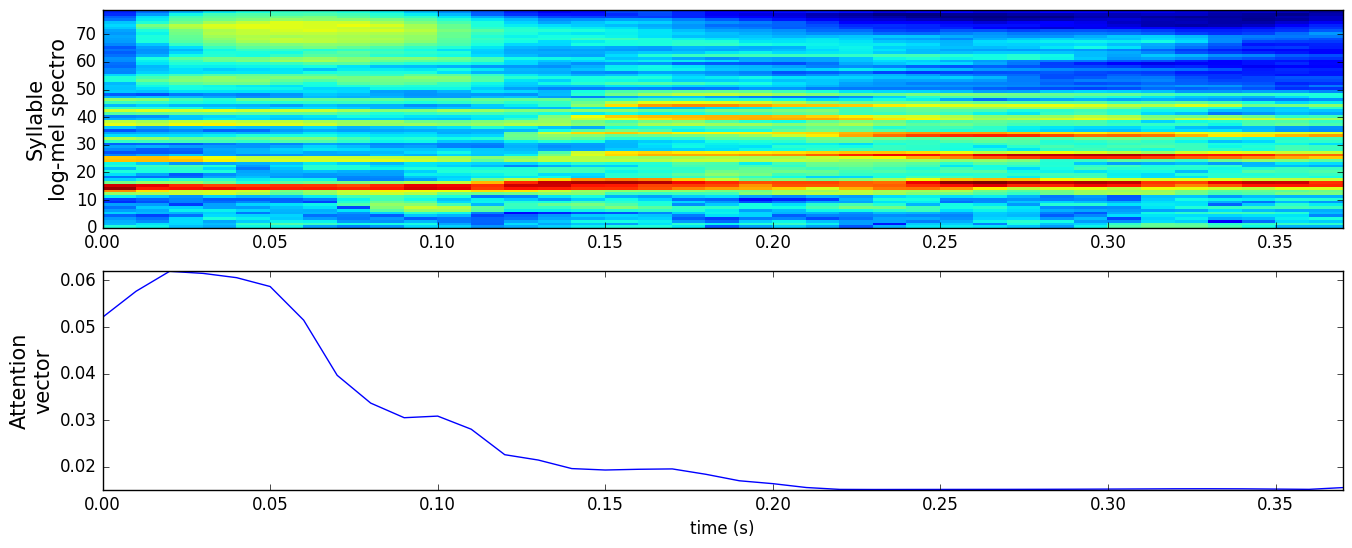
\includegraphics[width=0.475\textwidth]{figs/spectro_vis/ch6_jiantuanzi_0.png}}
        % \label{fig:ch4:c_laosheng}}
    \subfloat[Jiantuanzi 2]{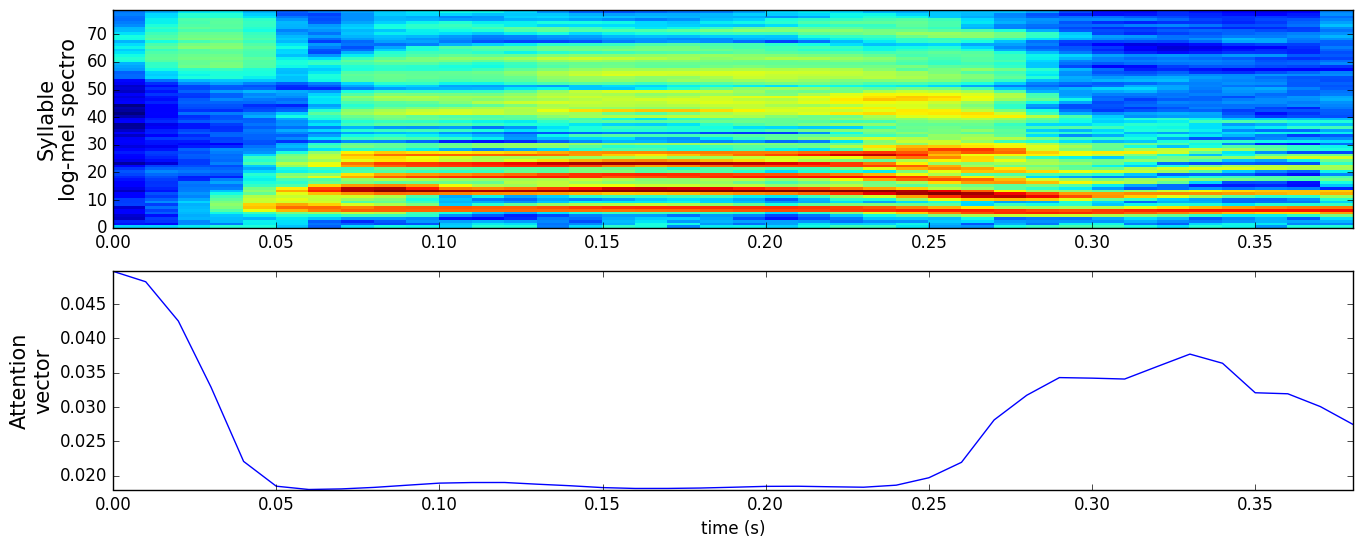
\includegraphics[width=0.475\textwidth]{figs/spectro_vis/ch6_jiantuanzi_1.png}}
        % \label{fig:ch4:l_laosheng}}
    \hfill

    \subfloat[Jiantuanzi 3]{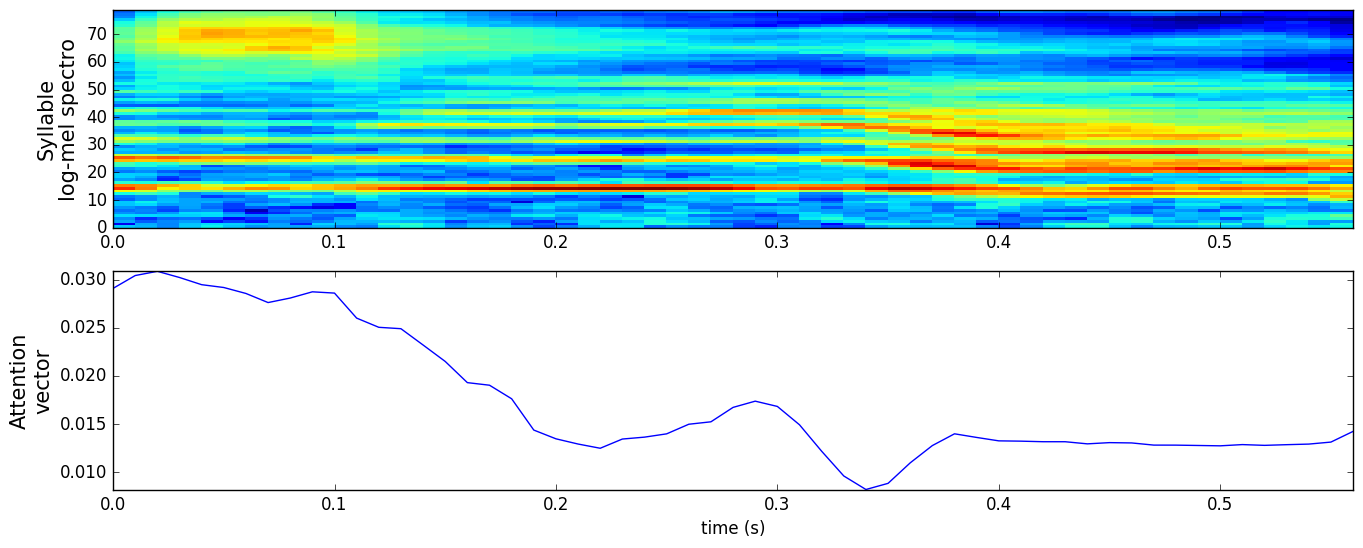
\includegraphics[width=0.475\textwidth]{figs/spectro_vis/ch6_jiantuanzi_2.png}}
        % \label{fig:ch4:N_laosheng}}
    \subfloat[Jiantuanzi 4]{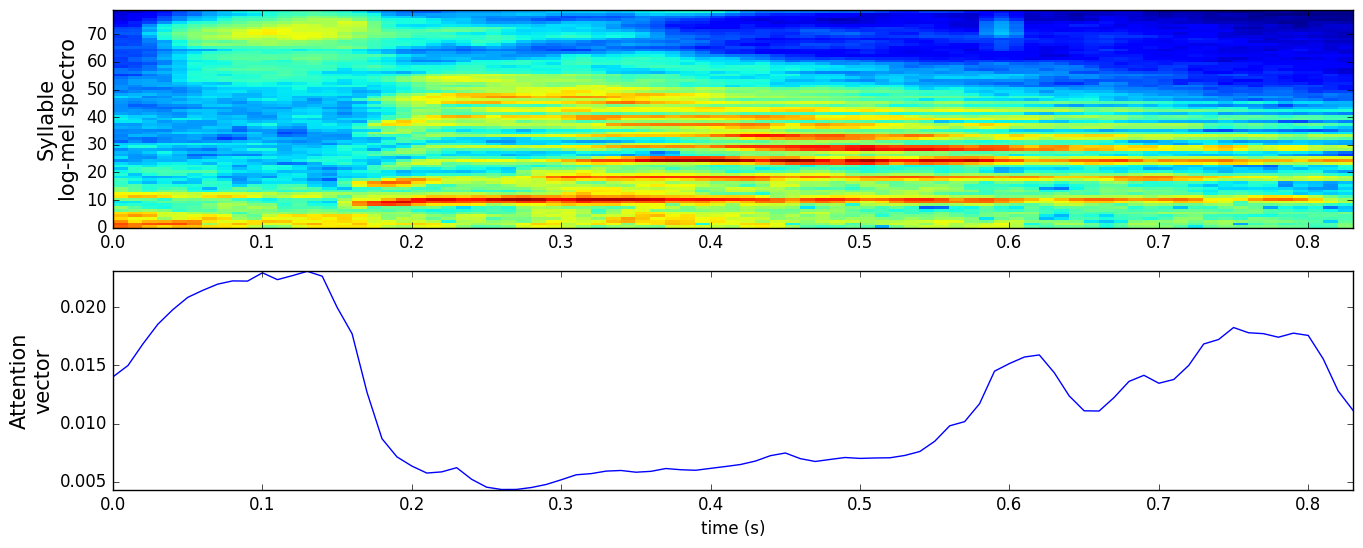
\includegraphics[width=0.475\textwidth]{figs/spectro_vis/ch6_jiantuanzi_3.png}}
        % \label{fig:ch4:@n_laosheng}}
    \hfill

    \subfloat[Jiantuanzi 5]{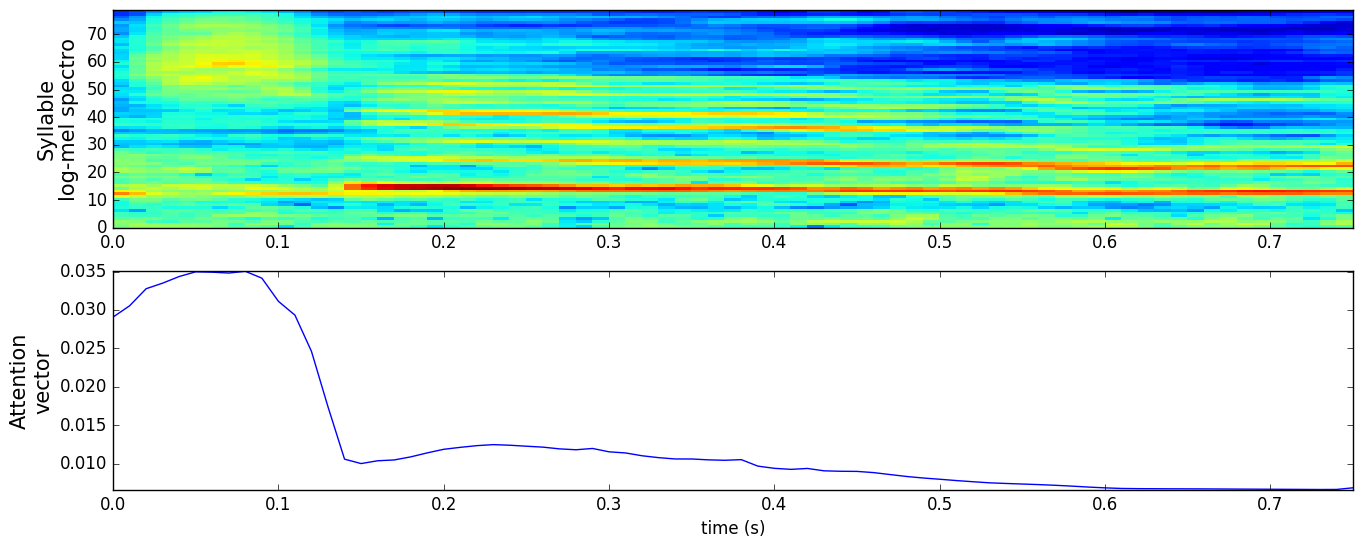
\includegraphics[width=0.475\textwidth]{figs/spectro_vis/ch6_jiantuanzi_4.png}}
        % \label{fig:ch4:i_laosheng}}
    \subfloat[Jiantuanzi 6]{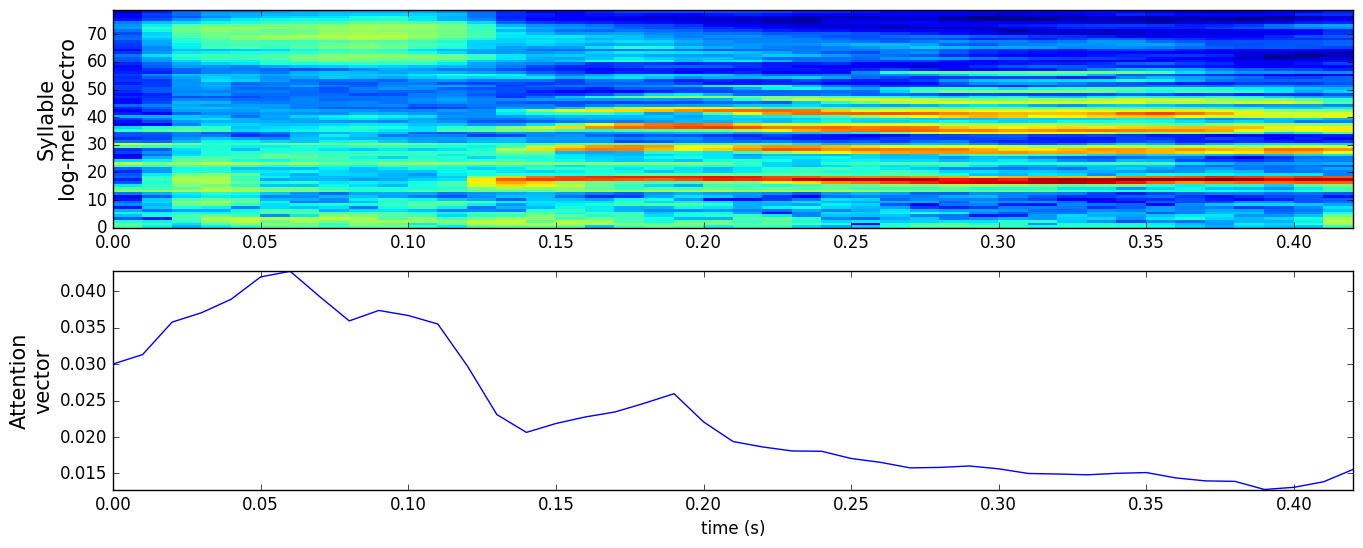
\includegraphics[width=0.475\textwidth]{figs/spectro_vis/ch6_jiantuanzi_5.png}}
        % \label{fig:ch4:a_laosheng}}
    \hfill

    \subfloat[Jiantuanzi 7]{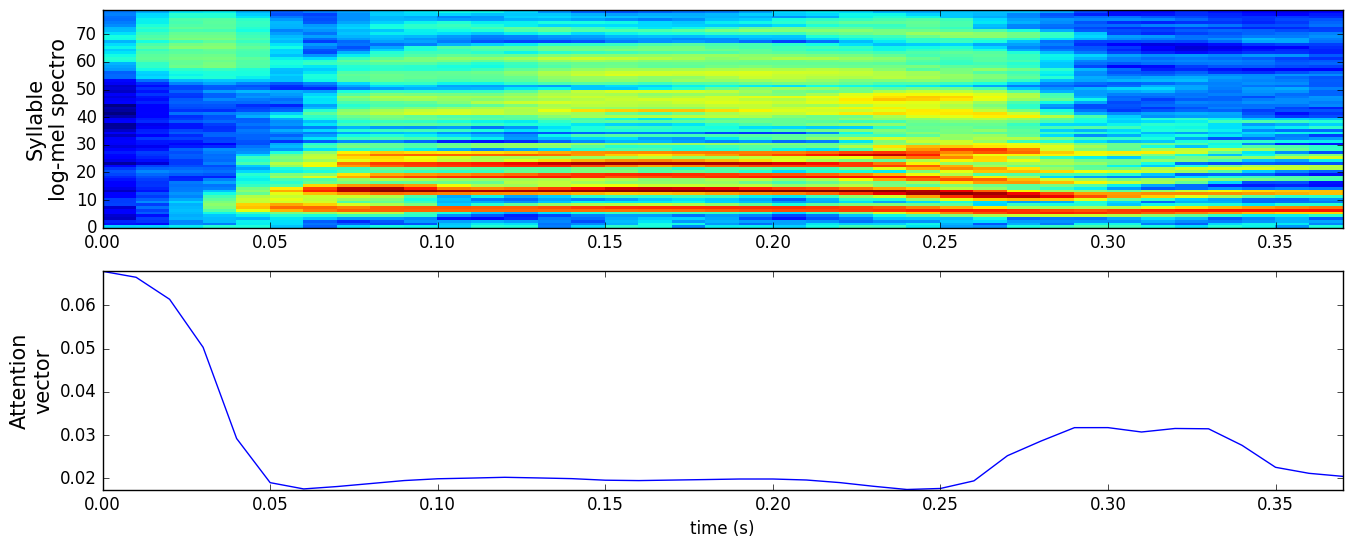
\includegraphics[width=0.475\textwidth]{figs/spectro_vis/ch6_jiantuanzi_6.png}}
        % \label{fig:ch4:i_laosheng}}
    \subfloat[Jiantuanzi 8]{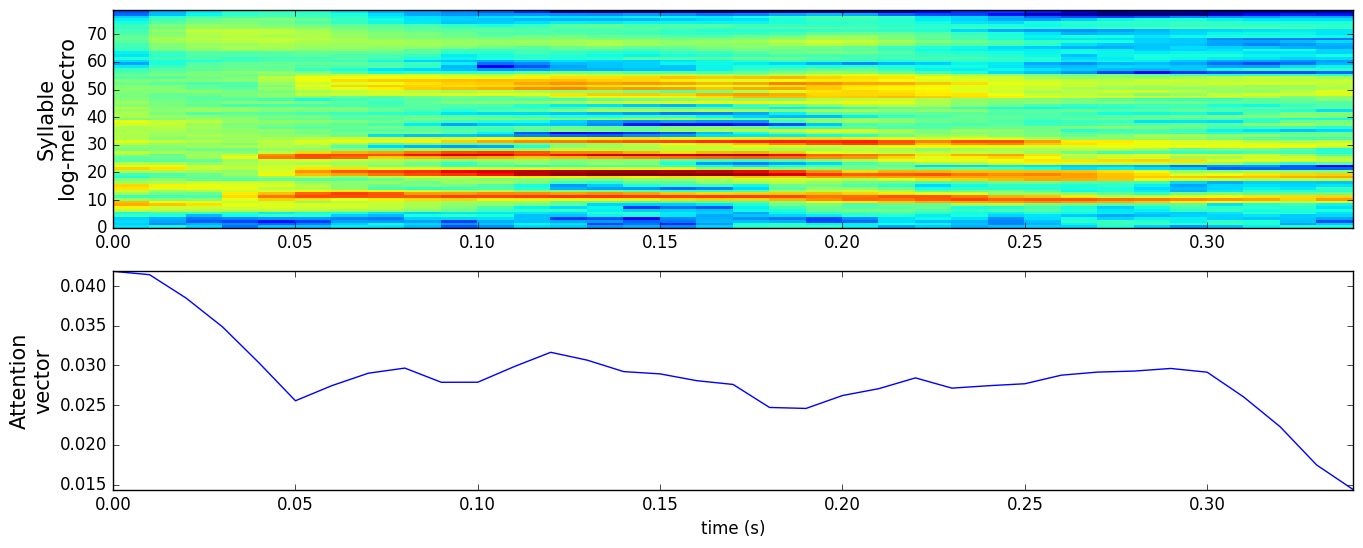
\includegraphics[width=0.475\textwidth]{figs/spectro_vis/ch6_jiantuanzi_7.png}}
        % \label{fig:ch4:a_laosheng}}
  
    \caption[]{The visualization of the logarithmic Mel spectrogram and the attention vector output from the model decoding process for jiantuanzi syllables.}
    \label{fig:ch6:jiantuanzi_att_vector}
\end{figure}


We can notice from \figref{fig:ch6:jiantuanzi_att_vector} that the attention vectors have a relatively high value towards the non-voiced consonant part of the syllable (the noise-like spectrogram at the syllable beginning), which means that the attention mechanism allows the model to make the decision mainly on the non-voiced consonant part of the syllable, which is the segment to discriminate a mispronounced and a correctly pronounced jiantuanzi syllable.

\section{Improving the discriminative mispronunciation detection models}

In the last section, we devised a discriminative model-based mispronunciation detection method. The discriminative model is based on deep learning architecture which classifies the input syllable segment binarily into mispronounced or correctly pronounced class. The classification accuracy largely depends on the deep learning architecture, the size and quality of training dataset. To collect more training data would involve the participation of multi-party, e.g., artists, recording engineers, which is more difficult in coordination and more time-consuming than experimenting new deep learning architectures. 

In this section, we experiment with two new deep learning architectures and intend to improve the mispronunciation accuracy. These two architectures have been proposed recently for the sequential data modelling.

\subsection{Temporal convolutional networks}

Temporal convolutional networks (TCNs) is a deep learning architecture proposed by Bai et al. \cite{Bai2018}. TCNs adopts three novel deep learning techniques -- causal convolutions, dilated convolutions and residual connections to perform sequential modelling rather than using RNN-related architectures. The author evaluated TCNs along with several traditional sequential modelling architectures, such as LSTM, GRU and RNN, on various sequential modelling tasks, such as polyphonic music modelling, word- and character-level language modelling. The experiment shows that TCNs outperformed those architectures in most of the tasks. The main component of the TCNs is a 1D full-convolutional network (FCN). The causal convolutions restrict that there can be no leakage of information from the future into the past. The dilated convolutions can achieve a large history size while maintaining a relatively small layer number (not too deep) and filter size (not too large). Residual connections can stabilize a large and deep network by only learning the modifications to the identity mapping. The memory retention analysis shows that TCNs exhibit substantially longer memory than the LSTMs and GRUs of the same size.

TCNs hold several hyperparameters which need to be tuned when applying the model to the mispronunciation detection task. The most important factor for choosing hyperparameters is to make sure the TCN has a sufficiently large receptive field to cover the amount of the sequential context. The relevant hyperparameters are the number of stacks $n$ of the FCN, dilation factor $d$ and filter size $k$. The receptive field size which is equal to $d\times k \times n$ needs to be adapted to the average syllable length of our training dataset -- 86.09 frames. We experiment with three hyperparameter configurations:

\begin{table}[ht!]
\centering
\caption{Configurations of three TCNs. $n$: number of stacks, $d$: dilation factor, $k$: filter size.}
\label{tab:ch6:tcns_configurations}
\begin{tabular}{ccccc}
\toprule
& \makecell[c]{Receptive field\\size (frames)} & $n$ & $k$ & $d$ for each stack \\
\midrule
TCNs1 & 8192 & 4 & 8 & [2, 4, 16, 256] \\
TCNs2 & 128 & 4 & 8 & [1, 2, 4, 16] \\
TCNs3 & 96 & 4 & 8 & [1, 2, 8, 32] \\
\bottomrule
\end{tabular}
\end{table}

\subsection{Self-attention mechanism}

The feed-forward attention mechanism presented in \secref{sec:ch6:feed_forward_att} aims to learn a fixed-length embedding vector by weighted summing the RNN hidden states of all timestamps. The attention vector is learned by a multilayer perceptron (MLP) model, which allows the model to emphasize certain hidden states. Lin et al. \cite{Lin2017} proposed a structured self-attention mechanism which learns a 2D embedding matrix rather than a vector. Applying for the natural language sentence embedding task, they claim that each row of the matrix can attend on a different part of the sentence. 

They argue that the feed-forward attention mechanism using an embedding vector usually focus on a specific component (time region) of the input sequence. To allow the model to attend to multiple components, they proposed to use multiple attention vectors, which forms an embedding matrix. Consequently, to compute the embedding matrix is to learn a weighting matrix of which each row is the weighting vector of the hidden state sequence. In the implementation, we use a 2-layer MLP without bias to learn this weighting matrix.

The theoretical framework of the self-attention mechanism is compelling, and also has practical meaning when applying to the mispronunciation detection. For example, when a student mispronounces a syllable, she/he might commit errors on multiple parts of the syllable. E.g., the mispronunciation of ``sian" could be ``xiang", where the student made the errors on both non-voiced consonant ``s" -> ``x" and the terminal consonant ``n" -> ``ng".

In this work, we experiment with the self-attention mechanism with the BiLSTM architecture presented in \secref{sec:ch6:bilstm}. To prevent overfitting, we restrict the number of parameters in the architecture and use 16 hidden units for each layer of the MLP.

\subsection{Experimental setup}

The experimental setup is the same as it has been mentioned in \secref{sec:ch6:experimental_setup}.

\subsection{Results and discussions}

\tabref{tab:ch6:results_tcns_val} shows the MVL results of three TCNs hyperparameter configurations. For special pronunciation task, the TCNs3 with the smallest receptive field size performs the best. While for jiantuanzi task, the TCNs1 with the largest receptive field size performs the best. The possible reason is that the model needs a large receptive field to retain the long history in order to detection the mispronunciation of a jianzi syllable, of which the mispronunciation usually happens at the non-voiced consonant part which is also the beginning of the syllable. While for special pronunciation task, the mispronunciation usually happens at the syllable belly or tail position, which doesn't require the model to have a large receptive field to retain the long history. However, the best results among the three configurations still lag behind those of the previous experimented BiLSTM models (\secref{tab:ch6:results_discriminative_val}), that we need a further study to understand the poor results of the TCNs. An assumption could be that TCNs requires more training data to work properly. However, our current training dataset is too small.

\begin{table}[ht!]
\centering
\caption{Mean validation loss (MVL) of three TCN hyperparameter configurations for special pronunciation and jiantuanzi detection tasks.}
\label{tab:ch6:results_tcns_val}
\begin{tabular}{cccc}
\toprule
& TCNs1 & TCNs2 & TCNs3 \\
\midrule
\makecell{MVL\\special} & 1.2831 & 1.1702 & 1.0787 \\
\makecell{MVL\\jiantuanzi} & 0.8877 & 0.9986 & 1.2243 \\
\#params & 14609 & 7505 & 8097 \\
\bottomrule
\end{tabular}
\end{table}

\tabref{tab:ch6:results_self_att_val} shows the MVL results of self-attention and feed-forward attention mechanism. We can observe an improvement by adopting self-attention, which means that using the self-attention mechanism individually with BiLSTM leads to a better performance than using feed-forward attention. However, we combining self-attention with other deep learning techniques mentioned in \secref{sec:ch6:discriminative_dl_models}, the performance for the special pronunciation task does not surpass the best result reported in \tabref{tab:ch6:results_discriminative_val}, and the performance for the jiantuanzi task is worse than using self-attention individually.

\begin{table}[ht!]
\centering
\caption{Mean validation loss (MVL) of self-attention and feed-forward attention architectures for special pronunciation and jiantuanzi detection tasks. Self-att.: self-attention, Feed-forward: feed-forward attention, Comb.: combine BiLSTM, CNN, self-attention and dropout.}
\label{tab:ch6:results_self_att_val}
\begin{tabular}{cccc}
\toprule
& Self-att. & Feed-forward & Comb. \\
\midrule
\makecell{MVL\\special} & 0.6458 & 0.6560 & 0.6313 \\
\makecell{MVL\\jiantuanzi} & 0.3512 & 0.3892 & 0.3943 \\
\#params & 6257 & 5730 & 9761 \\
\bottomrule
\end{tabular}
\end{table}

Because of the inferior results of TCNs and self-attention mechanism, we would not include them in the final models for the mispronunciation detection tasks. Consider that the relatively small training data size might be the bottleneck of improving the deep learning-based detection models, it is more reasonable to collect more training data firstly, then study the performance of different deep learning architectures.

\section{Conclusions} 

This chapter presented a detailed formulation of the task of mispronunciation detection in jingju singing voice. The approaches utilized the automatic syllable segmentation algorithm presented in the last chapter and a deep learning-based discriminative model to perform the detection on two types of jingju singing syllables. Evaluation on an amateur jingju singing dataset showed the possibility of this approach and its limitations. The goal of developing such model was to present a methodology for mispronunciation detection in automatic singing voice assessment system of jingju music. The work presented in this chapter was preliminary and not comprehensive, with a great possibility for further study and improvement. However, the basic idea of using a deep learning-based discriminative model to achieve the mispronunciation detection is valid.

We mainly addressed the problem of the detection of two types of mispronounced syllables in jingju singing recordings -- special pronunciation and jiantuanzi. The presented method firstly used the onset detection-based automatic syllable segmentation algorithm to obtain the segment of each syllable, then classified each syllable segment to mispronounced or correctly pronounced class by using a deep learning-based discriminative model. Compared to a baseline forced alignment method, we showed that the proposed method is more advantageous in detecting the mispronunciation of the jiantuanzi syllable type. By illustrating the attention vector, we found that the attention mechanism is useful in putting more weights in the non-voiced consonant part of, and thus to help the model to make a better detection of the jiantuanzi mispronunciation. Additionally, intending to improve the detection accuracy of the discriminative model, we adopted two newly developed deep learning techniques for sequential modelling to our mispronunciation detection task. However, the results showed that their performance was not ideal, and inferior to our initial discriminative model.

For future work, we aim to improve the discriminative model performance by collecting more training dataset. Deep learning techniques are known to be data-consuming. However, our current dataset for training the deep learning-based discriminative model is too small to train a proper discriminative model and to outperform the forced alignment-based model which usually requires much less training data. The next steps would be performing an extensive hyperparameter tuning for the deep learning models since the performance of such models can be optimized by considering the coordinative effect between the hyperparameters and the size of the training data.
